% Created by tikzDevice version 0.12.3.1 on 2022-03-15 02:59:11
% !TEX encoding = UTF-8 Unicode
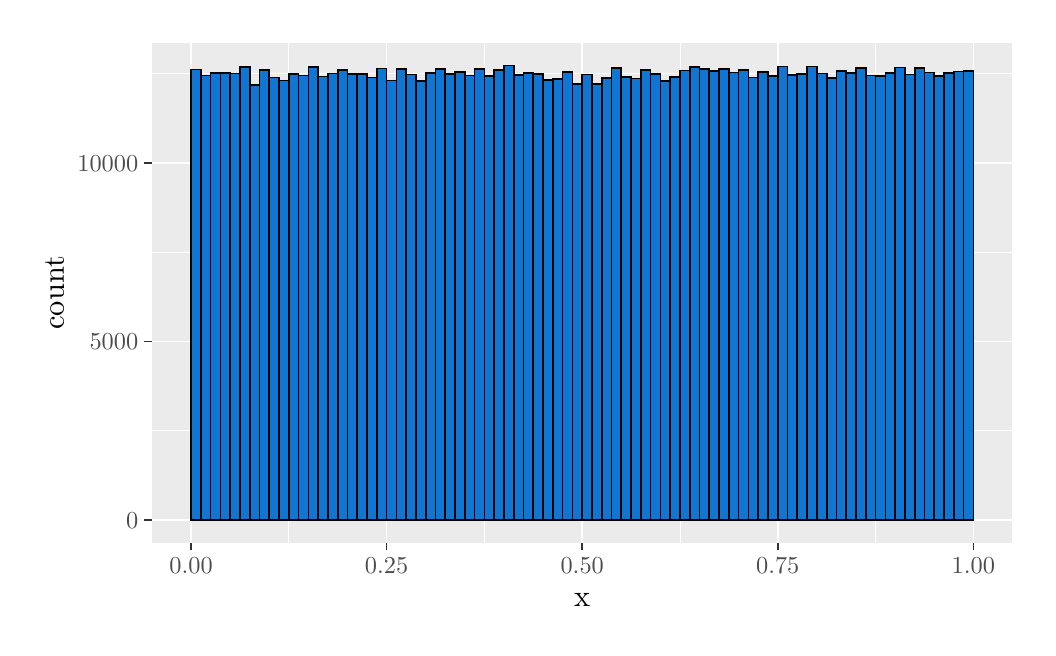
\begin{tikzpicture}[x=1pt,y=1pt]
\definecolor{fillColor}{RGB}{255,255,255}
\path[use as bounding box,fill=fillColor,fill opacity=0.00] (0,0) rectangle (361.35,216.81);
\begin{scope}
\path[clip] (  0.00,  0.00) rectangle (361.35,216.81);
\definecolor{drawColor}{RGB}{255,255,255}
\definecolor{fillColor}{RGB}{255,255,255}

\path[draw=drawColor,line width= 0.6pt,line join=round,line cap=round,fill=fillColor] (  0.00,  0.00) rectangle (361.35,216.81);
\end{scope}
\begin{scope}
\path[clip] ( 44.91, 30.69) rectangle (355.85,211.31);
\definecolor{fillColor}{gray}{0.92}

\path[fill=fillColor] ( 44.91, 30.69) rectangle (355.85,211.31);
\definecolor{drawColor}{RGB}{255,255,255}

\path[draw=drawColor,line width= 0.3pt,line join=round] ( 44.91, 71.16) --
	(355.85, 71.16);

\path[draw=drawColor,line width= 0.3pt,line join=round] ( 44.91,135.70) --
	(355.85,135.70);

\path[draw=drawColor,line width= 0.3pt,line join=round] ( 44.91,200.23) --
	(355.85,200.23);

\path[draw=drawColor,line width= 0.3pt,line join=round] ( 94.38, 30.69) --
	( 94.38,211.31);

\path[draw=drawColor,line width= 0.3pt,line join=round] (165.05, 30.69) --
	(165.05,211.31);

\path[draw=drawColor,line width= 0.3pt,line join=round] (235.71, 30.69) --
	(235.71,211.31);

\path[draw=drawColor,line width= 0.3pt,line join=round] (306.38, 30.69) --
	(306.38,211.31);

\path[draw=drawColor,line width= 0.6pt,line join=round] ( 44.91, 38.90) --
	(355.85, 38.90);

\path[draw=drawColor,line width= 0.6pt,line join=round] ( 44.91,103.43) --
	(355.85,103.43);

\path[draw=drawColor,line width= 0.6pt,line join=round] ( 44.91,167.97) --
	(355.85,167.97);

\path[draw=drawColor,line width= 0.6pt,line join=round] ( 59.04, 30.69) --
	( 59.04,211.31);

\path[draw=drawColor,line width= 0.6pt,line join=round] (129.71, 30.69) --
	(129.71,211.31);

\path[draw=drawColor,line width= 0.6pt,line join=round] (200.38, 30.69) --
	(200.38,211.31);

\path[draw=drawColor,line width= 0.6pt,line join=round] (271.05, 30.69) --
	(271.05,211.31);

\path[draw=drawColor,line width= 0.6pt,line join=round] (341.72, 30.69) --
	(341.72,211.31);
\definecolor{drawColor}{RGB}{0,0,0}
\definecolor{fillColor}{RGB}{16,118,212}

\path[draw=drawColor,line width= 0.6pt,line cap=rect,fill=fillColor] ( 59.04, 38.90) rectangle ( 62.58,201.64);

\path[draw=drawColor,line width= 0.6pt,line cap=rect,fill=fillColor] ( 62.58, 38.90) rectangle ( 66.11,199.58);

\path[draw=drawColor,line width= 0.6pt,line cap=rect,fill=fillColor] ( 66.11, 38.90) rectangle ( 69.64,200.31);

\path[draw=drawColor,line width= 0.6pt,line cap=rect,fill=fillColor] ( 69.64, 38.90) rectangle ( 73.18,200.42);

\path[draw=drawColor,line width= 0.6pt,line cap=rect,fill=fillColor] ( 73.18, 38.90) rectangle ( 76.71,200.22);

\path[draw=drawColor,line width= 0.6pt,line cap=rect,fill=fillColor] ( 76.71, 38.90) rectangle ( 80.24,202.65);

\path[draw=drawColor,line width= 0.6pt,line cap=rect,fill=fillColor] ( 80.24, 38.90) rectangle ( 83.78,196.18);

\path[draw=drawColor,line width= 0.6pt,line cap=rect,fill=fillColor] ( 83.78, 38.90) rectangle ( 87.31,201.56);

\path[draw=drawColor,line width= 0.6pt,line cap=rect,fill=fillColor] ( 87.31, 38.90) rectangle ( 90.84,198.76);

\path[draw=drawColor,line width= 0.6pt,line cap=rect,fill=fillColor] ( 90.84, 38.90) rectangle ( 94.38,197.69);

\path[draw=drawColor,line width= 0.6pt,line cap=rect,fill=fillColor] ( 94.38, 38.90) rectangle ( 97.91,200.16);

\path[draw=drawColor,line width= 0.6pt,line cap=rect,fill=fillColor] ( 97.91, 38.90) rectangle (101.44,199.52);

\path[draw=drawColor,line width= 0.6pt,line cap=rect,fill=fillColor] (101.44, 38.90) rectangle (104.98,202.58);

\path[draw=drawColor,line width= 0.6pt,line cap=rect,fill=fillColor] (104.98, 38.90) rectangle (108.51,199.11);

\path[draw=drawColor,line width= 0.6pt,line cap=rect,fill=fillColor] (108.51, 38.90) rectangle (112.04,200.25);

\path[draw=drawColor,line width= 0.6pt,line cap=rect,fill=fillColor] (112.04, 38.90) rectangle (115.58,201.56);

\path[draw=drawColor,line width= 0.6pt,line cap=rect,fill=fillColor] (115.58, 38.90) rectangle (119.11,200.07);

\path[draw=drawColor,line width= 0.6pt,line cap=rect,fill=fillColor] (119.11, 38.90) rectangle (122.64,200.07);

\path[draw=drawColor,line width= 0.6pt,line cap=rect,fill=fillColor] (122.64, 38.90) rectangle (126.18,198.81);

\path[draw=drawColor,line width= 0.6pt,line cap=rect,fill=fillColor] (126.18, 38.90) rectangle (129.71,202.02);

\path[draw=drawColor,line width= 0.6pt,line cap=rect,fill=fillColor] (129.71, 38.90) rectangle (133.24,197.73);

\path[draw=drawColor,line width= 0.6pt,line cap=rect,fill=fillColor] (133.24, 38.90) rectangle (136.78,201.95);

\path[draw=drawColor,line width= 0.6pt,line cap=rect,fill=fillColor] (136.78, 38.90) rectangle (140.31,199.94);

\path[draw=drawColor,line width= 0.6pt,line cap=rect,fill=fillColor] (140.31, 38.90) rectangle (143.84,197.50);

\path[draw=drawColor,line width= 0.6pt,line cap=rect,fill=fillColor] (143.84, 38.90) rectangle (147.38,200.54);

\path[draw=drawColor,line width= 0.6pt,line cap=rect,fill=fillColor] (147.38, 38.90) rectangle (150.91,201.90);

\path[draw=drawColor,line width= 0.6pt,line cap=rect,fill=fillColor] (150.91, 38.90) rectangle (154.45,200.02);

\path[draw=drawColor,line width= 0.6pt,line cap=rect,fill=fillColor] (154.45, 38.90) rectangle (157.98,200.72);

\path[draw=drawColor,line width= 0.6pt,line cap=rect,fill=fillColor] (157.98, 38.90) rectangle (161.51,199.56);

\path[draw=drawColor,line width= 0.6pt,line cap=rect,fill=fillColor] (161.51, 38.90) rectangle (165.05,201.76);

\path[draw=drawColor,line width= 0.6pt,line cap=rect,fill=fillColor] (165.05, 38.90) rectangle (168.58,199.36);

\path[draw=drawColor,line width= 0.6pt,line cap=rect,fill=fillColor] (168.58, 38.90) rectangle (172.11,201.63);

\path[draw=drawColor,line width= 0.6pt,line cap=rect,fill=fillColor] (172.11, 38.90) rectangle (175.65,203.10);

\path[draw=drawColor,line width= 0.6pt,line cap=rect,fill=fillColor] (175.65, 38.90) rectangle (179.18,199.76);

\path[draw=drawColor,line width= 0.6pt,line cap=rect,fill=fillColor] (179.18, 38.90) rectangle (182.71,200.47);

\path[draw=drawColor,line width= 0.6pt,line cap=rect,fill=fillColor] (182.71, 38.90) rectangle (186.25,200.09);

\path[draw=drawColor,line width= 0.6pt,line cap=rect,fill=fillColor] (186.25, 38.90) rectangle (189.78,197.78);

\path[draw=drawColor,line width= 0.6pt,line cap=rect,fill=fillColor] (189.78, 38.90) rectangle (193.31,198.20);

\path[draw=drawColor,line width= 0.6pt,line cap=rect,fill=fillColor] (193.31, 38.90) rectangle (196.85,200.72);

\path[draw=drawColor,line width= 0.6pt,line cap=rect,fill=fillColor] (196.85, 38.90) rectangle (200.38,196.53);

\path[draw=drawColor,line width= 0.6pt,line cap=rect,fill=fillColor] (200.38, 38.90) rectangle (203.91,199.83);

\path[draw=drawColor,line width= 0.6pt,line cap=rect,fill=fillColor] (203.91, 38.90) rectangle (207.45,196.34);

\path[draw=drawColor,line width= 0.6pt,line cap=rect,fill=fillColor] (207.45, 38.90) rectangle (210.98,198.52);

\path[draw=drawColor,line width= 0.6pt,line cap=rect,fill=fillColor] (210.98, 38.90) rectangle (214.51,202.13);

\path[draw=drawColor,line width= 0.6pt,line cap=rect,fill=fillColor] (214.51, 38.90) rectangle (218.05,199.05);

\path[draw=drawColor,line width= 0.6pt,line cap=rect,fill=fillColor] (218.05, 38.90) rectangle (221.58,198.47);

\path[draw=drawColor,line width= 0.6pt,line cap=rect,fill=fillColor] (221.58, 38.90) rectangle (225.11,201.41);

\path[draw=drawColor,line width= 0.6pt,line cap=rect,fill=fillColor] (225.11, 38.90) rectangle (228.65,200.03);

\path[draw=drawColor,line width= 0.6pt,line cap=rect,fill=fillColor] (228.65, 38.90) rectangle (232.18,197.60);

\path[draw=drawColor,line width= 0.6pt,line cap=rect,fill=fillColor] (232.18, 38.90) rectangle (235.71,198.92);

\path[draw=drawColor,line width= 0.6pt,line cap=rect,fill=fillColor] (235.71, 38.90) rectangle (239.25,201.38);

\path[draw=drawColor,line width= 0.6pt,line cap=rect,fill=fillColor] (239.25, 38.90) rectangle (242.78,202.66);

\path[draw=drawColor,line width= 0.6pt,line cap=rect,fill=fillColor] (242.78, 38.90) rectangle (246.31,201.89);

\path[draw=drawColor,line width= 0.6pt,line cap=rect,fill=fillColor] (246.31, 38.90) rectangle (249.85,201.23);

\path[draw=drawColor,line width= 0.6pt,line cap=rect,fill=fillColor] (249.85, 38.90) rectangle (253.38,201.76);

\path[draw=drawColor,line width= 0.6pt,line cap=rect,fill=fillColor] (253.38, 38.90) rectangle (256.91,200.63);

\path[draw=drawColor,line width= 0.6pt,line cap=rect,fill=fillColor] (256.91, 38.90) rectangle (260.45,201.53);

\path[draw=drawColor,line width= 0.6pt,line cap=rect,fill=fillColor] (260.45, 38.90) rectangle (263.98,198.80);

\path[draw=drawColor,line width= 0.6pt,line cap=rect,fill=fillColor] (263.98, 38.90) rectangle (267.51,200.78);

\path[draw=drawColor,line width= 0.6pt,line cap=rect,fill=fillColor] (267.51, 38.90) rectangle (271.05,199.24);

\path[draw=drawColor,line width= 0.6pt,line cap=rect,fill=fillColor] (271.05, 38.90) rectangle (274.58,202.75);

\path[draw=drawColor,line width= 0.6pt,line cap=rect,fill=fillColor] (274.58, 38.90) rectangle (278.11,199.77);

\path[draw=drawColor,line width= 0.6pt,line cap=rect,fill=fillColor] (278.11, 38.90) rectangle (281.65,200.09);

\path[draw=drawColor,line width= 0.6pt,line cap=rect,fill=fillColor] (281.65, 38.90) rectangle (285.18,202.83);

\path[draw=drawColor,line width= 0.6pt,line cap=rect,fill=fillColor] (285.18, 38.90) rectangle (288.72,200.27);

\path[draw=drawColor,line width= 0.6pt,line cap=rect,fill=fillColor] (288.72, 38.90) rectangle (292.25,198.52);

\path[draw=drawColor,line width= 0.6pt,line cap=rect,fill=fillColor] (292.25, 38.90) rectangle (295.78,201.05);

\path[draw=drawColor,line width= 0.6pt,line cap=rect,fill=fillColor] (295.78, 38.90) rectangle (299.32,200.53);

\path[draw=drawColor,line width= 0.6pt,line cap=rect,fill=fillColor] (299.32, 38.90) rectangle (302.85,202.20);

\path[draw=drawColor,line width= 0.6pt,line cap=rect,fill=fillColor] (302.85, 38.90) rectangle (306.38,199.52);

\path[draw=drawColor,line width= 0.6pt,line cap=rect,fill=fillColor] (306.38, 38.90) rectangle (309.92,199.32);

\path[draw=drawColor,line width= 0.6pt,line cap=rect,fill=fillColor] (309.92, 38.90) rectangle (313.45,200.34);

\path[draw=drawColor,line width= 0.6pt,line cap=rect,fill=fillColor] (313.45, 38.90) rectangle (316.98,202.40);

\path[draw=drawColor,line width= 0.6pt,line cap=rect,fill=fillColor] (316.98, 38.90) rectangle (320.52,199.86);

\path[draw=drawColor,line width= 0.6pt,line cap=rect,fill=fillColor] (320.52, 38.90) rectangle (324.05,202.24);

\path[draw=drawColor,line width= 0.6pt,line cap=rect,fill=fillColor] (324.05, 38.90) rectangle (327.58,200.63);

\path[draw=drawColor,line width= 0.6pt,line cap=rect,fill=fillColor] (327.58, 38.90) rectangle (331.12,199.31);

\path[draw=drawColor,line width= 0.6pt,line cap=rect,fill=fillColor] (331.12, 38.90) rectangle (334.65,200.42);

\path[draw=drawColor,line width= 0.6pt,line cap=rect,fill=fillColor] (334.65, 38.90) rectangle (338.18,200.92);

\path[draw=drawColor,line width= 0.6pt,line cap=rect,fill=fillColor] (338.18, 38.90) rectangle (341.72,201.19);
\end{scope}
\begin{scope}
\path[clip] (  0.00,  0.00) rectangle (361.35,216.81);
\definecolor{drawColor}{gray}{0.30}

\node[text=drawColor,anchor=base east,inner sep=0pt, outer sep=0pt, scale=  0.88] at ( 39.96, 35.87) {0};

\node[text=drawColor,anchor=base east,inner sep=0pt, outer sep=0pt, scale=  0.88] at ( 39.96,100.40) {5000};

\node[text=drawColor,anchor=base east,inner sep=0pt, outer sep=0pt, scale=  0.88] at ( 39.96,164.94) {10000};
\end{scope}
\begin{scope}
\path[clip] (  0.00,  0.00) rectangle (361.35,216.81);
\definecolor{drawColor}{gray}{0.20}

\path[draw=drawColor,line width= 0.6pt,line join=round] ( 42.16, 38.90) --
	( 44.91, 38.90);

\path[draw=drawColor,line width= 0.6pt,line join=round] ( 42.16,103.43) --
	( 44.91,103.43);

\path[draw=drawColor,line width= 0.6pt,line join=round] ( 42.16,167.97) --
	( 44.91,167.97);
\end{scope}
\begin{scope}
\path[clip] (  0.00,  0.00) rectangle (361.35,216.81);
\definecolor{drawColor}{gray}{0.20}

\path[draw=drawColor,line width= 0.6pt,line join=round] ( 59.04, 27.94) --
	( 59.04, 30.69);

\path[draw=drawColor,line width= 0.6pt,line join=round] (129.71, 27.94) --
	(129.71, 30.69);

\path[draw=drawColor,line width= 0.6pt,line join=round] (200.38, 27.94) --
	(200.38, 30.69);

\path[draw=drawColor,line width= 0.6pt,line join=round] (271.05, 27.94) --
	(271.05, 30.69);

\path[draw=drawColor,line width= 0.6pt,line join=round] (341.72, 27.94) --
	(341.72, 30.69);
\end{scope}
\begin{scope}
\path[clip] (  0.00,  0.00) rectangle (361.35,216.81);
\definecolor{drawColor}{gray}{0.30}

\node[text=drawColor,anchor=base,inner sep=0pt, outer sep=0pt, scale=  0.88] at ( 59.04, 19.68) {0.00};

\node[text=drawColor,anchor=base,inner sep=0pt, outer sep=0pt, scale=  0.88] at (129.71, 19.68) {0.25};

\node[text=drawColor,anchor=base,inner sep=0pt, outer sep=0pt, scale=  0.88] at (200.38, 19.68) {0.50};

\node[text=drawColor,anchor=base,inner sep=0pt, outer sep=0pt, scale=  0.88] at (271.05, 19.68) {0.75};

\node[text=drawColor,anchor=base,inner sep=0pt, outer sep=0pt, scale=  0.88] at (341.72, 19.68) {1.00};
\end{scope}
\begin{scope}
\path[clip] (  0.00,  0.00) rectangle (361.35,216.81);
\definecolor{drawColor}{RGB}{0,0,0}

\node[text=drawColor,anchor=base,inner sep=0pt, outer sep=0pt, scale=  1.10] at (200.38,  7.64) {x};
\end{scope}
\begin{scope}
\path[clip] (  0.00,  0.00) rectangle (361.35,216.81);
\definecolor{drawColor}{RGB}{0,0,0}

\node[text=drawColor,rotate= 90.00,anchor=base,inner sep=0pt, outer sep=0pt, scale=  1.10] at ( 13.08,121.00) {count};
\end{scope}
\end{tikzpicture}
